\section{Die \texorpdfstring{$\boldsymbol{uvw}$}{uvw}-Methode}\label{kapitel:uvw}
Die $uvw$-Methode ist eine Methode, um Ungleichungen in drei Variablen auf den Spezialfall zu reduzieren, dass eine Variable gleich $0$ ist oder dass zwei Variablen gleich sind. Zusammen mit einer Nebenbedingung (oder unter Ausnutzung von Homogenität) könnt ihr die Ungleichung dann weiter auf nur noch eine Variable reduzieren und spätestens an diesem Punkt habt ihr fast immer gewonnen. Die Methode ist überdies sehr flexibel und führt auch bei Ungleichungen mit untypischen Gleichheitsfällen zum Ziel, bei denen AM-GM oder Jensen zwangsläufig versagen würden.

Gegeben sei also eine Ungleichung in den drei\footnote{Wenn ihr den Beweis des $uvw$-Theorems verstanden habt, wird euch klar sein, dass die Methode auch für mehr als drei Variablen anwendbar ist. Nur seid ihr bei vier oder mehr Variablen noch nicht fertig, wenn ihr wisst, dass zwei Variablen gleich sein müssen. Um die Ungleichung weiter zu reduzieren, könntet ihr als nächstes zum Beispiel die Schiebemethode auf zwei der verbleibenden Variablen anwenden \ldots} Variablen $a,b,c\geqslant 0$, gerne auch mit einer Nebenbedingung. Wir substituieren
\begin{equation*}
	u=a+b+c\,,\quad v=ab+bc+ca\,,\quad w=abc
\end{equation*}
Häufig kommt es nun vor, dass die Ungleichung monoton in einer der Variablen $u$, $v$ und $w$ ist. In diesem Fall können wir die anderen beiden Variablen fixieren und müssen nur den Fall betrachten, dass die monotone Variable minimal oder maximal ist.\footnote{Dieses Argument funktioniert noch in weiteren Fällen. Zum Beispiel könnte es passieren, dass wir einen Ausdruck in $u$, $v$ und $w$ maximieren wollen, der in einer der drei Variablen konvex ist. Da konvexe Funktionen ihr Maximum immer am Rand des Definitionsbereiches annehmen, können wir wiederum die anderen beiden Variablen fixieren und die konvexe Variable minimieren oder maximieren.} Was bedeutet es nun, minimal oder maximal zu sein? Die einzige Einschränkung, die $u$, $v$ und $w$ erfüllen müssen, ist, dass das Polynom
\begin{equation*}
	p(X)=X^3-uX^2+vX-w=(X-a)(X-b)(X-c)
\end{equation*}
drei nichtnegative reelle Nullstellen hat, denn wir fordern ja, dass $a,b,c\geqslant 0$ nichtnegative reelle Zahlen sind. Diese Überlegung führt uns nun auf das folgende Theorem.
\begin{satzmitnamen}[Tejs' $\boldsymbol{uvw}$-Theorem]
	Seien $u$, $v$ und $w$ wie oben.
	\begin{enumerate}[label={$(\alph*)$},ref={$(\alph*)$}]
		\item Wir fixieren $u$ und $v$. Dann existiert ein maximales $w$ mit der Eigenschaft, dass das Polynom $p_w(X)=X^3-uX^2+vX-w$ drei nichtnegative reelle Nullstellen hat, und für dieses $w$ hat $p_w$ sogar eine Doppelnullstelle. Ebenso existiert ein minimales $w$ mit dieser Eigenschaft, und dieses $p_w$ hat eine Doppelnullstelle oder eine Nullstelle bei $X=0$.\label{behauptung:uv}
		\item Wir fixieren $u$ und $w$. Dann existiert ein maximales und ein minimales $v$ mit der Eigenschaft, dass das Polynom $p_v(X)=X^3-uX^2+vX-w$ drei nichtnegative reelle Nullstellen hat. Für diese Werte von $v$ hat $p_v$ sogar eine Doppelnullstelle.\label{behauptung:uw}
		\item Wir fixieren $v$ und $w$. Wenn $w>0$, dann existiert ein maximales und ein minimales $u$ mit der Eigenschaft, dass das Polynom $p_u(X)=X^3-uX^2+vX-w$ drei nichtnegative reelle Nullstellen hat. Für diese Werte von $u$ hat $p_u$ sogar eine Doppelnullstelle. Wenn $w=0$, dann hat $p_u$ eine Nullstelle bei $X=0$.\label{behauptung:vw}
	\end{enumerate}
\end{satzmitnamen}
\begin{proof}
	Wir beweisen nur \ref{behauptung:vw}; die anderen beiden Aussagen gehen analog. Im Fall $w=0$ ist klar, dass $p_u$ eine Nullstelle bei $X=0$ hat. Wir können uns also auf den Fall $w\neq0$ beschränken.
	
	
	Zu jedem $p_u$ betrachten wir die Funktion $f_u\colon \mathbb R_{>0}\rightarrow \mathbb R$, $f_u(x)=p_u(x)/x^2$. Wegen $w>0$ kann $p_u$ keine Nullstelle bei $x=0$ haben, also besitzen $p_u$ und $f_u$ die gleichen Nullstellen. Sei $u_0$ irgendein fester Wert von $u$, sodass $p_{u_0}$ drei nichtnegative Nullstellen hat; diese sind dann wegen $w>0$ automatisch positiv. Wir bezeichnen die Nullstellen mit $0<\alpha\leqslant \beta\leqslant \gamma$. Das Polynom $p_{u_0}$ ist dann nichtpositiv auf dem Intervall $(0,\alpha]$, nichtnegativ auf dem Intervall $[\alpha,\beta]$, wieder nichtpositiv auf dem Intervall $[\beta,\gamma]$ und schließlich wieder nichtnegativ auf dem Intervall $[\gamma,\infty)$. Selbiges gilt folglich auch für $f_{u_0}$. Weil $f_{u_0}$ außerdem stetig ist, nimmt es auf dem Intervall $[\alpha,\beta]$ einen maximalen Wert $\Delta^+$ und auf dem Intervall $[\beta,\gamma]$ einen minimalen Wert $\Delta^-$ an. 
	
	\begin{wrapfigure}{r}{0.51\textwidth}
		\centering\vspace{-0.5cm}
		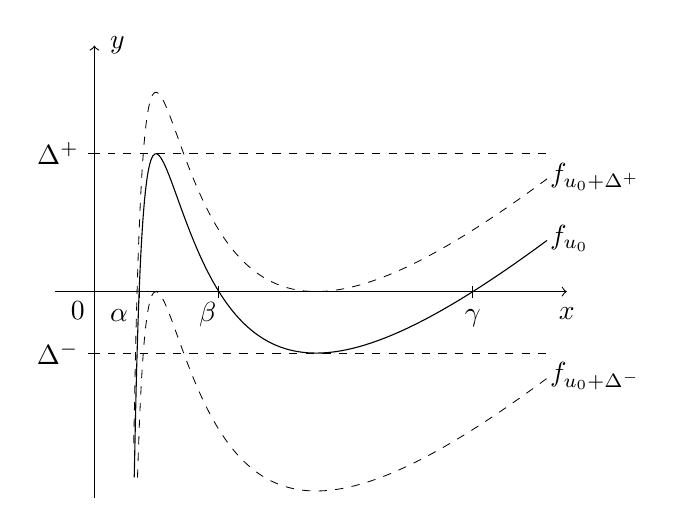
\begin{tikzpicture}[x=1.25cm,y=1.25cm]
			\draw[->] (-0.4,0) to node[pos=1,below=0.5ex] {$x$} (4.8,0);
			\draw[->] (0,-2.1) to  node[pos=1,right=0.5ex] {$y$} (0,2.5);
			\node[below left] at (0,0) {$0$};
			\draw plot[domain=0.28:4.475,smooth,samples=200] (\x+0.125,{(\x-0.33)*(\x-1.14)*(\x-3.72)/(\x*\x)});
			\draw[line width=0.3,dashed] plot[domain=0.313:4.5,smooth,samples=200] (\x+0.125,{(\x-0.33)*(\x-1.14)*(\x-3.72)/(\x*\x)-1.401});
			\draw[line width=0.3,dashed] plot[domain=0.275:4.5,smooth,samples=200] (\x+0.125,{(\x-0.33)*(\x-1.14)*(\x-3.72)/(\x*\x)+0.625});
			\draw (0,1.405) ++ (0.5ex,0) to ++(-1ex,0ex) node[left] {$\Delta^+$};
			\draw [line width=0.3,dashed,dash phase=0.5] (1.125ex,1.405) to (4.65,1.405);
			\draw (0,-0.629) ++ (0.5ex,0) to ++(-1ex,0ex) node[left] {$\Delta^-$};
			\draw [line width=0.3,dashed,dash phase=0.5] (1.125ex,-0.629) to (4.65,-0.629);
			\draw (0.455,0) ++ (0,0.5ex) to ++(0,-1ex);
			\draw (1.265,0) ++ (0,0.5ex) to ++(0,-1ex);
			\draw (3.845,0) ++ (0,0.5ex) to ++(0,-1ex);
			\node at (0.25,-0.24) {$\alpha$};
			\node at (1.15,-0.23) {$\beta\vphantom{\gamma}$};
			\node at (3.845,-0.23) {$\gamma\vphantom{\beta}$};
			\node[right=0.25ex] at (4.5,0.54) {$f_{u_0}$};
			\node[right=0.25ex] at (4.5,1.165) {$f_{u_0+\Delta^+}$};
			\node[right=0.25ex] at (4.5,-0.861) {$f_{u_0+\Delta^-}$};
		\end{tikzpicture}
	\end{wrapfigure}	
	Für beliebiges $u$ gilt stets
	\begin{equation*}
		f_u(x)=f_{u_0}(x)-(u-u_0)\,.
	\end{equation*}
	Daraus folgt, dass $f_u$ für $u>u_0+\Delta^+$ oder $u<u_0+\Delta^-$ nur eine reelle Nullstelle haben kann. Für diese Werte von $u$ hat also auch $p_u$ nur eine reelle Nullstelle. Im Fall $u=u_0+\Delta^+$ berührt hingegen der Graph von $f_{u_0+\Delta^+}$ die $x$-Achse irgendwo auf dem Intervall $[\alpha,\beta]$ (denn $\Delta^+$ war als Extremwert der differenzierbaren Funktion $f_{u_0}$ gewählt, deren Verschiebung um $-\Delta^+$ genau $f_{u+\Delta^+}$ ist), und schneidet sie ein weiteres Mal im Intervall $[\gamma,\infty)$. Selbiges muss also auch für $p_u$ gelten! Folglich hat $p_u$ drei positive reelle Nullstellen, wobei die ersten beiden zu einer Doppelnullstelle zusammenfallen.
	
	Das zeigt, dass $u=u_0+\Delta^+$ der maximale Wert ist, für den $p_u$ drei nichtnegative reelle Nullstellen hat, und wie wir gerade gesehen haben, hat $p_u$ dann sogar eine Doppelnullstelle, wie behauptet. Analog ist $u=u_0+\Delta^-$ der minimale Wert, für den $p_u$ drei nichtnegative reelle Nullstellen hat, und in genau der gleichen Weise erhalten wir, dass $p_u$ dann sogar eine Doppelnullstelle hat. Das zeigt die Behauptung.
\end{proof}


Wir werden die Methode nun an einer Aufgabe demonstrieren und euch zwei weitere  Beispielaufgaben stellen. Am Ende dieses Kapitels findet ihr Tipps und am Ende des Heftes findet ihr Musterlösungen zu den Beispielaufgaben.
\begin{aufgabe*}
	Man beweise, dass für alle nichtnegativen reellen Zahlen $x$, $y$, $z$ mit $x+y+z=1$ die folgende Ungleichung gilt:
	\begin{equation*}
		\frac{x}{1-yz}+\frac{y}{1-zx}+\frac{z}{1-xy}\leqslant\frac 98\,.
	\end{equation*}
\end{aufgabe*}
\begin{proof}[Lösung]
	Indem wir brutal mit allen Nennern durchmultiplizieren, erhalten wir die Ungleichung
	\begin{equation*}
		x+y+z-\sum x^2y+xyz\parens*{x^2+y^2+z^2}\leqslant \frac 98\parens*{1-\sum xy+xyz(x+y+z)-x^2y^2z^2}\,.
	\end{equation*}
	Wegen $x+y+z=1$ ist $\sum x^2y=(x+y+z)\sum xy-3xyz=\sum xy-3xyz=v-3w$ und $x^2+y^2+z^2=(x+y+z)^2-2\sum xy=1-2v$. Somit wird die obige Ungleichung zu
	\begin{equation*}
		0\leqslant \frac 98\parens*{1-v+w-w^2}-\parens*{1+3w-v+w-2wv}\,.
	\end{equation*}
	Und die rechte Seite ist linear in $v$! Wenn wir also $u=1$ und $w$ festhalten, nimmt die rechte Seite ihren minimalen Wert auf dem \enquote{Rand} an, sprich, wenn $v$ maximal oder minimal ist. Nach dem $uvw$-Theorem hat das Polynom $X^3-uX^2+vX-w=(X-x)(X-y)(X-z)$ in diesem Fall eine Doppelnullstelle. Das heißt, wir dürfen ohne Einschränkung $x=y$ annehmen. Wegen $x+y+z=1$ ist dann außerdem $z=1-2x$. Indem wir all das einsetzen, ausmultiplizieren und den offensichtlichen Gleichheitsfall $x=y=z=1$ ausklammern, erhalten wir die Ungleichung
	\begin{equation*}
		0\leqslant \frac18(3x-1)^2\parens*{-4x^4+12x^3-5x^2+4x+1}\,.
	\end{equation*}
	Für $0\leqslant x\leqslant 1$ ist $4x^4\leqslant 4x^3\leqslant 12x^3$ und $5x^2\leqslant 5x\leqslant 4x+1$, also ist der zweite Faktor auf der rechten Seite stets nichtnegativ. Der erste Faktor ist sowieso ein Quadrat. Also gilt die Ungleichung und wir sind fertig.
\end{proof}

\begin{aufgabe*}\label{aufgabe:DEMO2015Ungleichung}
	Beweise, dass für alle positiven reellen Zahlen $x,y,z>0$ die folgende Ungleichung gilt:
	\begin{equation*}
		\frac{x+y+z}{3}+\frac{3}{\frac1x+\frac1y+\frac1z}\geqslant 5\sqrt[3]{\frac{xyz}{16}}\,.
	\end{equation*}
\end{aufgabe*}
\begin{aufgabe*}[*]\label{aufgabe:UngleichungInvertieren}
	Gegeben seien nichtnegative reelle Zahlen $x,y,z\geqslant 0$ mit $x^2+y^2+z^2+2xyz=1$. Zeige, dass
	\begin{equation*}
		xy+yz+zx\leqslant \frac12+2xyz\,.
	\end{equation*}
\end{aufgabe*}

\subsection*{Tipps zu den Beispielaufgaben}
\textbf{Tipps zu Aufgabe~\ref{aufgabe:DEMO2015Ungleichung}.} Errate die Gleichheitsfälle (Spoiler: $x=y=z$ ist es nicht) und benutze die $uvw$-Methode.	

\textbf{Tipps zu Aufgabe~\ref{aufgabe:UngleichungInvertieren}.} Hier lässt sich die $uvw$-Methode nicht direkt anwenden, denn in der Nebenbedingung kommen sowohl $u$, $v$ als auch $w$ vor. Gibt es ein Argument, mit dem die Ungleichung und ihre Nebenbedingung vertauscht werden können? (Dieses Argument ist ein Trick, den ihr euch merken solltet!)

Es gibt bei dieser Aufgabe nicht nur den Gleichheitsfall $x=y=z=\frac12$. Errate die anderen Gleichheitsfälle.